% INIT + pakker
\documentclass[12pt, letterpaper]{article}
%\documentclass[twocolumn,11pt]{article}
\usepackage[margin=2 cm]{geometry}
\usepackage{latex_code/preamble}

\usepackage{makeidx}
\makeindex

%%%%%%%%%%%%% Frontpage
\title{TMA4267 - Linear statistical models}
\date{Spring semester 2024} 
\author{Trond Skaret Johansen}
\setcounter{secnumdepth}{3} % Adjust what sections are numbered

\begin{document}
\maketitle
\tableofcontents
\newpage

\section{Introduction} 

This is a brief summary of the course TMA4267 about linear statistical models. It includes the main content from the lecture held by \TODO{}... recorded in, where some examples etc... are excluded. 

The purpose of the notes is to give a good overview of the syllabus. I intend to add summaries of the lectures as I review them. I hope to include insights from projects / exercises where it is appropriate. 

\subsection*{Topics}
The first chapter begins by introducing multivariate distributions and how to compute expectations. We then move on to multivariate moments and transformations. Principal component analysis (PCA) is described, before we explain the need for charactestic functions and not just moment generating functions when working with multivariate distributions. 

In the second chapter we introduce the multivariate normal distribution. We deal with estimation in the multivariate normal distribution and give the theory of quadratic forms and idempotent matrices.

The third chapter tackles multiple linear regression. We introduce the model and its assumptions and estimate the parameters. Properties of the estimators, fitted values and residuals are established, and then put to use in performing inference about the coefficients. We perform t-tests, do ANOVA, compute the coefficient of determination and perform general F-tests. Finally, we look at some way of transforming the data.

In the fourth chapter, we analyse the model and the selection of models. We perform multiple hypothesis testing and present examples. 

In the fifth and final chapter, we do more ANOVA and investigate design of experiment. Our focus is two-level factorial design.
\label{sec:introduction}

% TODO: remove

\section*{Course progress} 

\begin{multicols}{3}
    \begin{itemize}
        \item First reading
        \begin{todolist}
            % \item[\done] Frame the problem
            \item[\done] Lecture 1-22
            \item Lecture 23
            \item Lecture 24
            \item Lecture 25
        \end{todolist}
        \item Gjennomgang
        \begin{todolist}
            \item[\done] Lecture 1-2
            \item Lecture 3-4
            \item Lecture 5-6
            \item[\done] Lecture 7-8
            \item Lecture 9-10
            \item Lecture 11-12
            \item Lecture 13-14
            \item Lecture 15-16
            \item Lecture 17-18
            \item Lecture 19-20
            \item Lecture 21-22
            \item Lecture 23
        \end{todolist}
    \end{itemize}
\end{multicols}


\subsection*{Exams}
\begin{multicols}{3}
    \begin{todolist}
        \item May 2023
        \item June 2019
        \item May 2018
        \item May 2017
        \item June 2016
        \item May 2015
        \item May 2014
        \item August 2014    
    \end{todolist}        
\end{multicols}

\subsection*{Topics}
\subsubsection*{1}
Multivariate distributions and expectations (HS 4.1-4.2).

Multivariate moments (HS 4.2 using HS 2.1-2.4).

Transformations (HS 4.3, 4.4)

PCA (HS 11.1-11.3).

Charactestic functions (HS 4.2). 


\subsubsection*{2}
Multivariate normal distribution (HS 4.4, 5.1).

Estimation in the multivariate normal distribution (HS 3.3, 4.5).

Quadratic forms and idempotent matrices (FKLM Appendix B, Th. B2, B8).


\subsubsection*{3}
Multiple linear regression: model, parameter estimation (FKLM 3.1, 3.2).

Properties of estimators, fitted values, residuals (FKLM 3.2). 

Inference about coefficients (FKLM 3.3).

Multiple linear regression: t-test about coefficients, ANOVA decomposition, coefficient of determination, F-test (FKLM 3.2, 3.3).

General F-test for regression coefficients (FKLM 3.2, 3.3, 3.5).

transformation of data (FKLM 3.2, 3.3, 3.4, 3.5).



\subsubsection*{4}
Model analysis and model selection (FKLM 3.4).

Multiple hypothesis testing (HBL).

Examples.


\subsubsection*{5}
ANOVA (HS 8.1.1). 

Design of experiment (DOE): two-level factorial design (T).

\subsection*{Keywords to know}


\newpage
\section{Multivariate Distribution and its Generalisations}
%%%%%%%%%%%%%%%%%%%%%%%%%%%%%%%%%%%%%%%%%%%%%
\subsection{Matrix algebra}

The main tool of the course is matrix algebra. We therefore repeat the most important convepts. The matrix $\mA$ is said to be \term{symmetric} if $\mA^\top=\mA$. It is \term{orthogonal} if $\mA\mA^\top=\mA^\top\mA=\mI$, i.e. if the columns are orthogonal. The elements of the pair ($\lambda, \boldsymbol{\gamma}$) are called \term{eigenvalue} and \term{eigenvector} respectivelly if they satisfy $\mA\boldsymbol{\gamma}=\lambda \boldsymbol{\gamma}$ and $\boldsymbol{\gamma}\ne \zero$. $\lambda$ can be found as the solution of $\det(\mA-\lambda \mI)$. Recall that the \term{trace}, $\tr{\mA}$, of a matrix is the sum of the diagonal. We also have the formulas:
$$
    \det{\mA} = \prod_{i=1}^p \lambda_i
    \quad
    \tr{\mA} = \sum_{i=1}^p \lambda_i.
$$
For a symmetric matrix we may find the \term{Jordan decomposition}. Let $\Lambda = \textrm{diag}\{\lambda_1, \dots, \lambda_p\}$ and $\Gamma = (\boldsymbol{\gamma_1}, \dots, \boldsymbol{\gamma_p})$. Then we have:
$$
    \mA=\mG\mL\mG^\top.
$$
For a symmetrix matrix $\mA$ and a vector $\x$ we define the \term{quadratic form}:
$$
    Q(\x) = \x^\top \mA \x = \sum_{i=1}^p\sum_{j=1}^p x_i A_{ij} x_j.
$$
\begin{theorem}
    Transforming $\y=\mG^\top\x$ we obtain 
    $$
        Q(\x) = \sum_{i=1}^p \lambda_i y_i^2.
    $$
\end{theorem}
A matrix is said to be \term{positive definite} if $Q(\x)>0$ for all $\x\ne0$ and positive semi definite if $Q(\x)\geq0$ for all $\x\ne0$. We write $A>0$ and $A\geq 0$ respectivelly. 
\begin{theorem}
    The symmetric matrix $A$ is positive definite iff $\lambda_i > 0$ for all $i$.
\end{theorem}
\begin{proof}
    Using the transform of the previous theorem we find 
    $$
        \lambda_1 y_1^2 + \dots + \lambda_p y_p^2 > 0 \quad\forall \y\in\R^p \Leftrightarrow \lambda_i > 0 \quad\forall i. 
    $$
\end{proof}
From this we obtain two more usefull results. 
\begin{enumerate}
    \item If $A>0$ the inverse exists and the determinant is $>0$
    \item If $A>0$ there exists a unique positive definite square root with decomposition:
    $$
        A^{1/2} = \mG\mL^{1/2}\mG^\top.
    $$
\end{enumerate}

%\subsection*{Lecture 1}
%%%%%%%%%%%%%%%%%%%%%%%%%%%%%%%%%%%%%%%%%%%%%%%%%%%%%%%%
\subsection{Random vectors and distributions}

A \term{random vector} $\X$ is a vector where each component is a \term{random variable}. Similarly, we define a \term{random matrix} as a matrix with random variables as component. As in the univariate case, we define the \term{cumulative distribution function} (CDF) by:
$$
    F(x)=\p{\X\leq \x} = \p{X_1\leq x_1,\dots,X_p\leq x_p}.
$$
A random vector is said to be \term{absolutelly continuous} if there exists a \term{probability density function} (PDF) $f$ such that:
$$
    F(\x)=\int_{-\infty}^{x_p}\dots\int_{-\infty}^{x_1} f(u_1,\dots,u_p) du_1\dots du_p.
$$
Then, we may compute the probability of the event $\X\in D$ by:
$$
    \p{\X\in D} = \int_D f(\x) d\x \quad\forall D\subseteq \R^p.
$$
The random cector is said to be \term{discrete} if it is consentraded on a countable (finite or infinite) set of points. Then integral becomes a sum. 

In the absolutelly continuous case, we may write the density as:
$$
    f(\x)=f\left(x_1, \ldots, x_p\right)=\frac{\partial^p F\left(x_1, \ldots, x_p\right)}{\partial x_1 \cdots \partial x_p}.
$$

Let $\X_A, \X_B$ be two random vectors st. $\X=(\X_A,\X_B)^\top$ has cdf $F$. Then we may find the \term{marginal distribution}:
$$
    F_A(x_1,\dots,x_k) = F(x_1,\dots,x_k,\infty,\dots,\infty).
$$
In absolutelly continuous case we find the marginal density:
$$
    f_A(x_1,\dots,x_k) = \int_{-\infty}^{\infty}\dots\int_{-\infty}^{\infty} f(x_1,\dots,x_p) du_p\dots du_{k+1}
$$

The \term{conditional distribution} of $\X_B$ given $\X_A = \x_A$ is:
$$
    f_{\X_B|\X_A=\x_A}(\x_B) = \frac{f(x_1,\dots,x_p)}{f_A(x_1,\dots,x_k)}
$$

We say that the random vectors $\X_A, \X_B$ are \term{independent} if 
$$
    F(x_1,\dots,x_p)=F_A(x_1,\dots,x_k)F_B(x_{k+1},\dots,x_p) \qall x_1,\dots x_p.
$$
In the continuous case we have independence iff $f=f_A\cdot f_B$. In this case $f_{\x_B|\X_A=\x_A} = f_B(\x_B)$.
Similar definition for independence when $\X$ has $N$ components and not just 2.

%%%%%%%%%%%%%%%%%%%%%%%%%%%%%%%%%%%%%%%%%%%%%%%%%%%%%%%%
\subsection{Multivariate expecations and moments}

We define the \term{expectation} of the random vector $\X$ as
$$
    \ev{\X} = (\ev{X_1},\dots,\ev{X_p})^\top.
$$
Here, each $\ev{X_i}=\int_{\R^p} x_i f(\x)d\x$. It is easy to show:
%\subsection*{Lecture 2}
\begin{enumerate}
    \item For constants $a,b$ we have $\ev{a \X + b \Y} = a\ev{\X}+ b \ev{\Y}$.
    \item For (shape compatible) matrices $\mA, \mB$ we have
    $
        \ev{\mA\X \mB} = \mA\ev{\X}\mB
    $.
    \item Let $\X, \Y$ be \emph{independent} random matrices whose product is defined. Then $\ev{\X\Y} = \ev{\X}\ev{\Y}$.   
\end{enumerate}        

Let $\X=(X_1,\dots,X_p)^\top$ and $\ev{\X}=:\M=({\mu_1,\dots,\mu_p})$. We then define the \term{covariance matrix} of $\X$ as:
$$
    \var{\X} = \cov{\X} = \SS = \begin{pmatrix}
        \sigma_{X_1X_1} & \dots & \sigma_{X_1X_p} \\
        \vdots & \ddots & \vdots \\
        \sigma_{X_pX_1} & \dots & \sigma_{X_pX_p}
    \end{pmatrix}
    =\ev{(\X-\M)(\X-\M)^\top}.
$$
This matrix is \term{symmetric}. Note also that $\SS_{ij}=\cov{X_i, X_j}$. We can also show:
$$
    \SS = \ev{\X\X^\top} - \M\M^\top.
$$
The correlation matrix (with ones on the diagonal as $\rho_{X_iX_i}=1$) is given by
$$
    \boldsymbol{\rho}
    =
    \begin{pmatrix}
        \rho_{X_1X_1} & \dots & \rho_{X_1X_p} \\
        \vdots & \ddots & \vdots \\
        \rho_{X_pX_1} & \dots & \rho_{X_pX_p}
    \end{pmatrix}
    ,\quad
    \rho_{X_iX_j} = \frac{\sigma_{X_iX_j}}{\sqrt{\sigma_{X_i}}\sqrt{\sigma_{X_j}}}.
$$
For two random vectors $\X,\Y$ we define their covariance matrix by
$$
    \SS_{\X\Y} 
    = \cov{\X,\Y} 
    = \ev{(\X-\M_{\X})(\Y-\M_{\Y})^\top}
    =(\cov{X_i,X_j})_{\substack{i=1,\dots,p \\ j= 1,\dots,q}}
$$

\begin{proposition}
    The covariance matrix $\SS$ is positive semi-definite.
\end{proposition}
\begin{proof}
    Using the formula for the variance of a linear combination we obtain:
    \begin{align*}
        \y^\top \SS \y 
        &= 
        \begin{pmatrix}
        y_1 & \cdots & y_n
        \end{pmatrix}
        \begin{pmatrix}
        \Sigma_{11} & \Sigma_{12} & \cdots & \Sigma_{1n} \\
        \Sigma_{21} & \Sigma_{22} & \cdots & \Sigma_{2n} \\
        \vdots & \vdots & \ddots & \vdots \\
        \Sigma_{n1} & \Sigma_{n2} & \cdots & \Sigma_{nn}
        \end{pmatrix}
        \begin{pmatrix}
        y_1 \\
        y_2 \\
        \vdots \\
        y_n
        \end{pmatrix}
        = \sum_{i=1}^{n} \sum_{j=1}^{n} y_i \Sigma_{ij} y_j
        \\&= \sum_{i=1}^{n} y_i^2 \text{Var}(X_i) + 2 \sum_{i < j} y_i y_j \text{Cov}(X_i, X_j)
        = \text{Var}\left( \sum_{i=1}^{n} y_i X_i \right)
        \geq 0. 
    \end{align*}
    Which completes the proof.
\end{proof}

\begin{remark}
    We usually require that the covariance matrix is \term{positive definite}, since if it is only positive semi-definite there are nontrivial linear combinations with 0 variance. Indeed, if 
    $\SS=\begin{pmatrix}
        1 & 1 \\ 1 & 1
    \end{pmatrix}$
    we obtain using the formula for variance of linear combinations that:
    $$
        \var{X_1 - X_2} = 1^2 \var{X_1} + (-1)^2 \var{X_2} + 2(1)(-1) \cov{X_1, X_2} = 0.
    $$
    This never happens for positive definite matrices since we for any nontrivial linear combination have:
    $$
        \cov{\boldsymbol{c}^\top \X} = \boldsymbol{c}^\top \SS \boldsymbol{c} > 0.
    $$        
\end{remark}

We have many more properties of covariance matrices:
\begin{enumerate}
    \item $\SS_{\X\Y} = \SS_{\Y\X}^\top$.
    \item If $\X\sim(\M_{\X}, \SS_{\X\X}), \Y\sim(\M_{\Y}, \SS_{\Y\Y})$ then $\Z=(\X,\Y)^\top$ has
    $$
        \SS_{\Z\Z} = \begin{pmatrix}
            \SS_{\X\X} & \SS_{\X\Y} \\ \SS_{\Y\X} & \SS_{\Y\Y}
        \end{pmatrix}.
    $$
    \item Independence of $\X,\Y$ implies $\cov{\X,\Y}=\zero$ (NB: the converse not true).
    \item $\var{\mA\X+\boldsymbol{b}} = \mA \var{\X}\mA^\top$.
    %\subsection*{Lecture 3}
    \item $\cov{\X+\Y, \Z} = \cov{\X, \Z} + \cov{\Y, \Z}$.
    \item $\var{\X+\Y} = \var{\X} + \cov{\X, \Y} + \cov{\Y, \Z} + \var{\Y}$.
    \item $\cov{\mA\X, \mB\Y} = \mA\cov{\X, \Y}\mB^\top$.
\end{enumerate}

%%%%%%%%%%%%%%%%%%%%%%%%%%%%%%%%%%%%%%%%%%%%%%%%%%%%%%%%
\subsection{Transformations}
\subsubsection{Mahalanobis transformation}

Our first transformation is the \term{Mahalanobis transformation}. We recall that we can get 0 mean and unit variance in the univariate case by the transformation $Y=\frac{X-\mu}{\s}$. In the multivariate case, suppose $X=(X_1,\dots, X_p)^\top\sim (\M, \SS)$ with $\SS$ non-singular. Then using the unique positive definite square root $\SS^{1/2}$ og $\SS$, we have the transformation:
\begin{equation}
    \boxed{\Y=\SS^{-1/2}(\X-\M) \sim (0, \mI)}
\end{equation}
\begin{proof}
    Compute the expected value and variance.
\end{proof}

%%%%%%%%%%%%%%%%%%%%%%%%%%%%%%%%%%%%%%%
\subsubsection{Principal component analysis (PCA)}
In the following we suppose that we observe realisations of some random vector $\X=(X_1,\dots,X_p)^\top \sim (\M, \SS)$. The goal of \term{principal component analysis} is to reduce dimensionality by removing some components and keeping components with large variance and hence more information. 

The idea is to first perform the transform $\X \mapsto \Y = \mA \X + \mb = (Y_1,\dots,Y_p)^\top$ in such a way that:
\begin{enumerate}
    \item $\ev{\Y} = \zero$,
    \item $\cov{Y_i, Y_j} = 0$ for $i\ne j$, i.e. $\SS_{\Y}$ is diagonal,
    \item $\var{Y_1} \geq \var{Y_2} \geq \dots \geq \var{Y_p}$.
\end{enumerate}
Using again the Jordan decomposition we may find such a transform. Arange $\SS = \boldsymbol{\Gamma}\boldsymbol{\Lambda}\boldsymbol{\Gamma}^\top$ such that the eigenvalues on the diagonal of $\boldsymbol{\Lambda} = \textrm{diag}\{\lambda_1, \dots, \lambda_p\}$ are ordered decreasingly. A transformation satisfying the requirements is then $\Y = \boldsymbol{\Gamma}^{1/2}(\X - \M)$. Indeed we may compute $\var{\Y} = \boldsymbol{\Lambda}$. We call $Y_1,\dots, Y_p$ the \term{principal components}. 

For the interpretation, recall that for the trace of a matrix we have:
$
    \tr{\mA\mB\mC}=\tr{\mB\mC\mA}=\tr{\mC\mA\mB}. 
$
Using this we compute:
\begin{align*}
    \textrm{\hermetegn{total variance}} 
    = \sum_{i=1}^p \var{X_i}
    = \tr{\SS}
    = \tr{\boldsymbol{\Gamma}\boldsymbol{\Lambda}\boldsymbol{\Gamma}^\top}
    = \tr{\boldsymbol{\Lambda}\boldsymbol{\Gamma}^\top\boldsymbol{\Gamma}}
    = \tr{\boldsymbol{\Lambda}}
    = \sum_{i=1}^n \lambda_i.
\end{align*}
Since we care about variability in our data, we can use this interpretation to extract the features explaining as much cariance as possible. For example we can keep the $m$ first principal components. Say we compute:
$$
    \frac{\sum_{i=1}^m\lambda_i}{\sum_{i=1}^p\lambda_i} = 0.8.
$$
Then we may say that \hermetegn{80\% of variability is explained by the components}, and we have succesfully reduced dimensionality. 

We can also do \term{empirical PCA} (also called \term{sample PCA}). Suppose that we have $n$ observations of independent identically distributed random vectors
$
    \X_i = \begin{pmatrix}
    X_{i1}, \ldots, X_{ip}
    \end{pmatrix}^\top \sim N(\mu, \Sigma)
$.
Gather them in a ($n\times p$) \hermetegn{data matrix}:
$$
    \X = \begin{pmatrix}
    \X_1^\top \\
    \X_2^\top \\
    \vdots \\
    \X_n^\top
    \end{pmatrix}
    = \begin{pmatrix}
    X_{11} & \cdots & X_{1p} \\
    X_{21} & \cdots & X_{2p} \\
    \vdots & \ddots & \vdots \\
    X_{n1} & \cdots & X_{np}
    \end{pmatrix}.
$$
Estimate the unknown $\M, \SS$ by $\bar{\X} = \frac{1}{n} \sum_{i=1}^n \X_i$ and $\boldsymbol{S} = \frac{1}{n-1} \sum_{j=1}^n (\X_i-\bar{\X})(\X_i-\bar{\X})^\top$. Then we may transform the matrix $\X$ into $\Y=(\X-\one_n \bar{\X})\boldsymbol{G}$ where $\boldsymbol{S}=\boldsymbol{G}\boldsymbol{L}\boldsymbol{G}$ is the Jordan decomposition of $\boldsymbol{S}$ with eigenvalues ordered decreasingly. Finally remove lowest components. 

\begin{remark}
    Intuitivelly, PCA can be though of as finding a $p$-dimensional ellipsoid that fits the data. The axis of the ellipsoid represent the principal components.

    \begin{figure}[H]
        \centering
        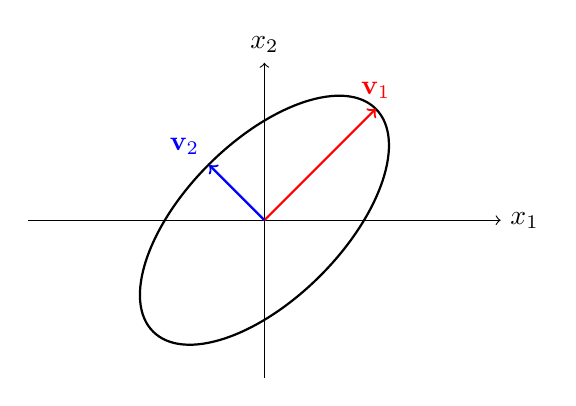
\begin{tikzpicture}
            % Draw the axes
            \draw[->][black] (-3,0) -- (3,0) node[right] {$x_1$};
            \draw[->][black] (0,-2) -- (0,2) node[above] {$x_2$};
            
            % Draw the ellipse
            \draw[black][rotate around={45:(0,0)}, thick] (0,0) ellipse (2 and 1);
            
            % Draw principal components
            \draw[->, red, thick] (0,0) -- (1.414, 1.414) node[above] {$\mathbf{v}_1$};
            \draw[->, blue, thick] (0,0) -- (-0.7, 0.7) node[above left] {$\mathbf{v}_2$};
            
        \end{tikzpicture}
        \caption{Principal Component Analysis (PCA) Ellipsoid. The red arrow indicates the first principal component (eigenvectors) $\mathbf{v}_1$ and the blue arrow indicates the second principal component $\mathbf{v}_2$.}
        \label{fig:pca_ellipsoid}
    \end{figure}
    
\end{remark}

%%%%%%%%%%%%%%%%%%%%%%%%%%%%%%%%%%%%%%%
\subsubsection{General transformations}

Suppose we transform the random vector $\X=(X_1,\dots,X_p)^\top$ into $\Y=g(\X)$. If the function $g$ is one-to-one and has differentiable inverse $u$, then 
\begin{equation*}
    f_{\Y}(\y) = |\det{\boldsymbol{J}}| f_{\X} (u(\y))
\end{equation*}
where 
$$
    \boldsymbol{J} = \brac{\frac{\partial u_i (y)}{\partial y_j}}_{i,j=1,\dots,p}
$$
is the \term{Jacobian matrix}. An important special case is that of linear transformations $\Y = \mA\X + \mb$. If $\mA$ is non-singular the inverse transform is $\X = \mA^{-1}(\Y-\mb)$ and $\boldsymbol{J} = \mA^{-1}$, so we obtain:
\begin{equation*}
    f_{\Y}(\y) = |\det{\mA^{-1}}| f_{\X} (\mA^{-1}(\y-\mb)).
\end{equation*}

%%%%%%%%%%%%%%%%%%%%%%%%%%%%%%%%%%%%%%%
%\subsection*{Lecture 4}
\subsection{Characteristic function}

In the univariate case we often studied the \term{moment generating function}:
$$
    M_X(t) = \ev{e^{tX}}.
$$
Important properties include:
\begin{enumerate}
    \item $M_X = M_Y \Rightarrow X \overset{d}{=} Y$,
    \item $\ev{X^k} = M^{(k)}_X(0)$,
    \item Independence of $X, Y$ implies $M_{X+Y} = M_X M_Y$.
\end{enumerate}
However, it does noe exist for for instance the student-t distribution. It only exists when all moments exist. We shall now define the \term{characteristic function}, which \textbf{always} exists:
$$
    \phi_X(t) = \ev{e^{itX}}.
$$
It has similar properties:
\begin{enumerate}
    \item $\phi_X = \phi_Y \Rightarrow X \overset{d}{=} Y$,
    \item $\ev{X^k} = i^{-k} \phi^{(k)}(0)$,
    \item Independence of $X, Y$ implies $\phi_{X+Y} = \phi_X \phi_Y$.
\end{enumerate}
In the p-variate case, the functions are functions of $\mt=(t_1,\dots,t_p)^\top$. Let as usual $\X=(X_1,\dots,X_p)^\top$ be our random vector. We define:
\begin{align*}
    M_{\X}(\mt) = \ev{e^{\mt^\top \X}}, \\
    \phi_{\X}(\mt) = \ev{e^{i\mt^\top \X}}.
\end{align*}
We list some important properties.
\begin{enumerate}
    \item If $\phi_{\X}(t)$ is absolutelly integrable, the (Fourier) inversion formula holds:
    $$
        f_{\X} = \frac{1}{(2\pi)^p} \int_{\R} e^{-i\mt^\top\x} \phi_{\X}(t) dt.
    $$
    \item Denote $t_{(1)} = (t_1,\dots,0)^\top, \dots, t_{(p)}=(0,\dots,t_p)^\top$. Then 
    $$
        \phi_{\X_k}(t_k) = \ev{e^{it_1 X_1}} = \ev{e^{i\mt_{(1)}^\top \X}} =  \phi_{\X}(t_{(k)}).
    $$
    \item Let $\X=\begin{pmatrix} \X_1 \\ \X_2 \end{pmatrix}$ and $\mt=\begin{pmatrix} \mt_1 \\ \mt_2 \end{pmatrix}$ be vectors with appropriate dimensions. Then:
    \begin{equation}
        \boxed{\X_1, \X_2 \textrm{ are independent } \Leftrightarrow \phi_{\X}(\mt) = \phi_{\X_1}(\mt_1)\phi_{\X_2}(\mt_2)}
    \end{equation} 
    \item Let $\X, \Y$ be independent p-variate random vectors. Then:
    $$
        \phi_{\X+\Y}(\mt) = \phi_{\X}(\mt)\phi_{\Y}(\mt).
    $$
\end{enumerate}
We end the section with a theorem linking the distributions of 1D random variables to the distribution of the p-variate random vector $\X$:
\begin{theorem}
    \term{Cramer-Wold} theorem states that the distribution of $\X\in\R^p$ is completelly determined by the set of all 1D distributions of $\mt^\top\X, \mt\in\R^p$.
\end{theorem}
\begin{proof}
    Suppose that for all $\mt\in\R^p$ we have $\mt^\top \X \overset{d}{=} \mt^\top \Y$. Then:
    $$
        \mt^\top \X \overset{d}{=} \mt^\top \Y \Rightarrow \phi_{\mt^\top\X}(u) = \phi_{\mt^\top\Y}(u).
    $$
    Taking $u=1$ gives $\ev{e^{i\mt^\top\X}} = \ev{e^{i\mt^\top\Y}}$ for all $\mt$, so $\phi_{\X}=\phi_{\Y}$ and hence $\X \overset{d}{=}  \Y$.
\end{proof}
\section{The Multivariate Normal Distribution}

%%%%%%%%%%%%%%%%%%%%%%%%%%%%%%%%%%%%%%%
\subsection{From univariate to multivariate}
\subsubsection{Univariate case}

We begin by recalling important properties and results of the univariate normal distribution. Let $-\infty<\mu<\infty, \s\geq 0$. We say $X\sim N(\mu,\s^2)$ if it has density:
$$
    f_X(x) = \frac{1}{\sqrt{2\pi \s^2}} e^{-\frac{1}{2}\brac{\frac{x-\mu}{\sigma}}^2}.
$$
The case $\s=0$ is considered normal degenerate and we have $X\overset{\mathrm{a.s.}}{=}\mu$. One can show $\ev{X}=\mu, \var{X}=\s^2$ and that the moment generating and characteristic functions are:
\begin{align*}
    M_X(t) &= e^{\mu t + \frac{\s^2 t^2}{2}}, \\
    \phi_X(t) &= e^{i\mu t - \frac{\s^2 t^2}{2}}.
\end{align*}
We say that $Z\sim N(0, 1)$ is standard normal. We can transform as follows:
\begin{align*}
    X \sim N(\mu, \s^2) &\Rightarrow \frac{X-\mu}{\s} \sim N(0,1), \\
    Z \sim N(0,1) &\Rightarrow \s Z + \mu \sim N(\mu, \s^2).
\end{align*}
A final fundamental property is that linear combinations of independent normal random variables are also normal. 


%%%%%%%%%%%%%%%%%%%%%%%%%%%%%%%%%%%%%%%
\subsubsection{Multivariate case}

We choose to present one of several equivalent definitions. Here we first define a special case and then generalise it. 
\begin{definition}
    A p-variate random vector $\Z=(Z_1, \dots, Z_p)^\top$ is a \term{standard normal vector} if its components are independent and each $Z_i\sim N(0,1)$. We imediatelly obtain $f_{\Z}(\z) = \prod f_{Z_i} (z_i)$. We use the notation $Z\sim N(0, \mI)$.
\end{definition}
\begin{definition}
    We say that $\X = (X_1,\dots, X_p)^\top$ is \term{multivariate normal} if there exists a ($p\times q$) matrix $\mA$ and $\M\in\R^p$ such that 
    $$
        \X = \mA \Z + \M, \quad \Z \sim (0, \mI_q).
    $$
\end{definition}
\begin{theorem}
    For any vector $\mb\in\R^p$ we have that $\mb^\top \X$ is a univariate normal random variable.
\end{theorem}
\begin{proof}
    It is a linear combination of independent normal random variables:
    $$
        \mb^\top \X = \mb^\top(\mA\Z + \M) = \mb^\top \mA \Z + \mb^\top\M \sim N. 
    $$
\end{proof}
From the definition we find $\ev{\X} = \M, \var{\X} = \mA\mA^\top =: \SS$. We write $\X \sim N(\M, \SS)$. It turns out that the statement from the theorem would give an equivalent definition!
%\subsection*{Lecture 5}
\begin{theorem}
    Let $\X \sim N(\M, \SS)$. If $\SS > 0$, then the probability density function (PDF) of $\X$ is:
    \begin{equation}
        \boxed{
            f_{\X} (\x) = \frac{1}{(2\pi)^{k/2}\det(\SS)^{1/2}} e^{-\frac{1}{2}(\x-\M)^\top\SS^{-1}(\x-\M)}
        }        
    \end{equation}
\end{theorem}
\begin{proof}
    Recall that $\X = \SS^{1/2}\Z + \M$. Using this, the result follows from the transformation formula and using the pdf of the standard normal $\Z$.  
\end{proof}
 
\begin{theorem}
    \label{thm:lin_comb}
    \begin{equation}
        \boxed{
            \X 
            \sim N(\M, \SS) \Rightarrow 
            \Y = 
            \mA\X+\boldsymbol{b} 
            \sim N(\mA\M+ \boldsymbol{b}, \mA \SS \mA^\top)
        }        
    \end{equation}
\end{theorem}
\begin{proof}
    Compute expected value and covariance. Normality follows from definition as we may write $\Y = \mA(\mB \Z + \boldsymbol{c}) + \boldsymbol{b} = \tilde{\mB} \Z + \tilde{\boldsymbol{b}}$. 
\end{proof}
The following corollary tells us that we may \term{standardize} in the multivariate case as well:
\begin{corollary}
    \begin{equation}
        \boxed{
            \X 
            \sim N(\M, \SS) \Rightarrow 
            \Z = 
            \SS^{-1/2}(\X-\M) 
            \sim N(0, \mI)
        }        
    \end{equation}
\end{corollary}
\begin{corollary}
    Any subvector $\X^*$ of $\X\sim N(\M, \SS)$ is also normal.
\end{corollary}
\begin{proof}
    Take $\mA$ to be a \hermetegn{component removing} matrix and use \Cref{thm:lin_comb}. 
\end{proof}

\begin{theorem}
    The characteristic function of $\X\sim N(\M, \SS)$ is:
    \begin{equation}
        \boxed{\phi_{\X}(\mt) = e^{ i \mt^\top\M - \frac{1}{2}\mt^\top\SS\mt}}
    \end{equation}
\end{theorem}
\begin{proof}
    For $Z\sim N(\zero, \mI_p)$, we may use independence to obtain:
    $$
        \phi_{\Z}(\mt) = \prod_{i=1}^p \phi_{Z_i}(t_i) = e^{-\frac{1}{2} \mt^\top\mt}.
    $$
    Then write $\X=\SS^{1/2} \Z + \M$ and rewrite:
    \begin{align*}
        \phi_{\X}(\mt) 
        &= \ev{e^{i\mt^\top\X}}
        = e^{i\mt^\top}\ev{e^{i\mt^\top\SS^{1/2}\Z}}
        = e^{i\mt^\top}\phi_{\Z}(\SS^{1/2}\mt)
        = e^{i\mt^\top}e^{-\frac{1}{2} \mt^\top\SS\mt}.
    \end{align*}
    Where we have used symmetry of $\SS^{1/2}$ a few times.
\end{proof}
The following is among the most important results in the course:
\begin{theorem}
    Suppose $\X\sim N(\M, \SS)$. Then 
    \begin{equation}
        \boxed{\mA \X, \mB \X \textrm{ are independent } \Leftrightarrow \cov{\mA \X, \mB \X} = \mA\SS\mB^\top = \zero}
    \end{equation} 
\end{theorem}
\begin{proof}
    The rightward implication is true for any random vectors. To prove the leftward for normal $\X$ we show that we may factor the characteristic function 
    $$
    \phi_{\begin{pmatrix}
        \mA \X \\ \mB \X
    \end{pmatrix}} (\mt) 
    = \phi_{\mA\X} (\mt_1) \phi_{\mB\X} (\mt_2).
    $$
    %\TODO{details if time, lecture 6}
\end{proof}
\begin{corollary}
    Let $X = (X_1,\dots,X_p)^\top\sim N{\M, \SS}$. Then $X_i, X_j$ independent iff $\cov{X_i,X_j}=0$.
\end{corollary}
\begin{remark}
    An important warning is that in the above all the $X_i$'s are jointly normal. The result is not true for any normally distributed $X_1, X_2$. Consider for example $X_1\sim N(0,1)$ and $X_2 = C X_1$ where C is a bernoulli distributed random variable with $P(C=1) = P(C=-1) = \frac{1}{2}$. Then also $X_2\sim N(0,1)$ and we find $\cov{X_1,X_2}=\ev{X_1X_2}=0$, but we do not have independence since $P(|X_1| \ne |X_2|) = 0$.  
    % https://math.stackexchange.com/questions/4076553/is-multinormality-required-for-zero-covariance-to-imply-independence
\end{remark}
The next theorem tells us that we may \hermetegn{remove the dependent part} of a component from another:
\begin{theorem}
    Let $\X\sim N(\M, \SS)$ be $p$-variate and $\X=(\X_1,\X_2)^\top$ with $\X_i\sim N(\M_i, \SS_i)$. Define $\X_2' = \X_2 - \SS_{21}\SS_{11}^{-1} \X_1$ Then:
    \begin{enumerate}
        \item $X_2'\sim N(\M_2 - \SS_{21}\SS_{11}^{-1}\M_1, \SS_{22} - \SS_{21}\SS_{11}^{-1}\SS_{12})$.
        \item $\X_1, \X_2'$ are independent.
    \end{enumerate}
\end{theorem}

\begin{theorem}
    With notation as in the previous theorem, the conditional distribution of $\X_2$ given $\X_1=\x_1$ is:
    \begin{equation}
        \boxed{
            \X_2 |_{\X_1 = \x_1} \sim N(\M_2 + \SS_{21}\SS_{11}^{-1}(\x_1-\M_1), \SS_{22}-\SS_{21}\SS_{11}^{-1}\SS_{12})
        }    
    \end{equation}
\end{theorem}

\begin{theorem}
    If $\X\sim N(\M, \SS)$ and $\SS$ is non-singular. Then 
    \begin{equation}
        \boxed{U = (\X-\M)\SS^{-1}(\X-\M) \sim \chi^2_p}        
    \end{equation}
\end{theorem}
\begin{proof}
    By definition of the $\chi^2$-distribution we have $U=\Z^\top\Z=Z_1^2+\dots+Z_p^2 \sim \chi_p^2$ for $\Z\sim N(0, \mI_p)$. By the \term{Mahalanobis transformation} we have $\Z=\SS^{\frac{1}{2}}(\X-\M)$ from which the result follows. 
\end{proof}


%\subsection*{Lecture 7}
%%%%%%%%%%%%%%%%%%%%%%%%%%%%%%%%%%%%%%%%%%%%%%%%%%%%%%%%%%%%%%%%%%
\subsection{Estimation of the multivariate normal distribution}
%%%%%%%%%%%%%%%%%%%%%%%%%%%%%%%%%%%%%%%%%%%%%%%%%%%%%%%%%%%%%%%%%%
\subsubsection{Univariate case}
From the univatiate case we recall that if $X_1,\dots,X_n \sim N(\mu, {\s^2})$ are independent, then the MLE estimators are:
\begin{align*}
    \mh &= \bar{X} = \frac{1}{n} \sum_{i=1}^n X_i, \\
    \sh^2 &= \frac{1}{n} \sum_{i=1}^n (X_i-\bar{X})^2.
\end{align*}
But since we found that $\ev{\s^2}=\frac{n-1}{n} \s^2$ is biased, we use instead the estimator
$$
    S^2 = \frac{1}{n-1} \sum_{i=1}^n (X_i-\bar{X})^2.
$$
We further proved that
\begin{enumerate}
    \item $\bar{X} \sim N(\mu, \s^2/n)$,
    \item $\frac{(n-1)S^2}{\s^2} \sim \chi^2_{n-1}$,
    \item $\bar{X}, S^2$ are independent (for the normal distribution),
    \item $\sqrt{n} \frac{\bar{X}-\mu}{S} \sim t_{n-1}$ (student t distribution).
\end{enumerate}
Our next goal is to obtain the result for the multivariate case. 

%%%%%%%%%%%%%%%%%%%%%%%%%%%%%%%%%%%%%%%%%%%%%%%%%%%%%%%%%%%%%%%%%%
\subsubsection{Multivatiate case}
In this case, we have $p$-variate independent randum vectors $\X_1,...,\X_n \sim N(\M, \SS)$ where we denote $\X_i=(X_{i1},\dots,X_{ip})^\top$. These make up the columns of the ($n\times p$) \term{data matrix} or \term{feature matrix} $\X$ given as:
$$
    \X = 
    \underset{\mr{features} \rightarrow}{
    \begin{pmatrix}
        X_{11} & \cdots & X_{1p} \\
        \vdots & \ddots & \vdots \\
        X_{n1} & \cdots & X_{np}
    \end{pmatrix}}
    \substack{\text{samples} \\ \downarrow}
    = \begin{pmatrix}
        \X_1^\top \\ \vdots \\ \X_n^\top
    \end{pmatrix}= (\X_1 \cdots \X_n)^\top.
$$
We want to estimate $\M, \SS$. Again we denote:
\begin{align*}
    \Mh &= \bar{\X} = \frac{1}{n} \sum_{i=1}^n \X_i = \frac{1}{n}\X^\top \one, \\
    \bs{S}^2 
    &= \frac{1}{n} \sum_{i=1}^n (\X_i-\bar{\X})(\X_i-\bar{\X})^\top 
    = \frac{1}{n} \X^\top\brac{\mI-\frac{1}{n} \one\one^\top}\X \TODO{?}.
\end{align*}
The matrix $\mC=\mI-\frac{1}{n} \one\one^\top$ is called the \term{centering matrix} because its action is to remove the mean of a vector:
$$
    \mC \y = \begin{pmatrix}
        1-\frac{1}{n} & \cdots & \frac{1}{n} \\
        \vdots & \ddots & \vdots \\
        \frac{1}{n} & \cdots & 1-\frac{1}{n}
    \end{pmatrix}
    \begin{pmatrix}
        y_1 \\ \vdots \\ y_n
    \end{pmatrix}
    = 
    \begin{pmatrix}
        y_1-\bar{y} \\ \vdots \\ y_n-\bar{y}
    \end{pmatrix}.
$$
We note that 
\begin{enumerate}
    \item $\mC$ is symmetric.
    \item $\mC$ is idempotent.
\end{enumerate}
For the estimators, we may prove:
\begin{proposition}
    $\bar{\X} \sim N(\M, \frac{1}{n}\SS)$
\end{proposition}
\begin{proof}
    The proof is by factoring the characteristic function. We can do this since the $\X_i$'s are independent.
    \begin{align*}
        \varphi_{\bar{\X}}(\mt) 
        &= \ev{e^{i \mt^\top \bar{\X}}}
        = \ev{ e^{i \left(\frac{\mt}{n}\right)^\top (\X_1, \ldots, \X_n)} }
        = \phi_{\X_1+\dots+\X_n} \left(\frac{\mt}{n}\right)
        = \varphi_{\X_1} \left( \frac{\mt}{n} \right) \cdots \varphi_{x_n} \left( \frac{\mt}{n} \right)
        \\&= \prod_{i=1}^{n} e^{ i \left(\frac{\mt}{n}\right)^\top\M - \frac{1}{2} \left(\frac{\mt}{n}\right)^\top \SS \left(\frac{\mt}{n}\right)^\top }
        = e^{\sum_{j=1}^{n} i \left(\frac{\mt}{n}\right)^\top\M - \frac{1}{2} \left(\frac{\mt}{n}\right)^\top \SS \left(\frac{\mt}{n}\right)^\top}
        = e^{ i \mt^\top \mu - \frac{1}{2} \mt^\top \frac{\SS}{n} \mt }.
    \end{align*}

\end{proof}
\begin{proposition}
    $\ev{\bs{S}} = \frac{n-1}{n} \SS.$
\end{proposition}
\begin{proof}
    This is a more straigh forward computation.
\end{proof}
Hence we obtain an unbiased estimator as
$$
    \bs{S}^2 = \frac{1}{n-1} \sum_{i=1}^n (\X_i-\bar{\X})(\X_i-\bar{\X})^\top.
$$

%\subsection*{Lecture 8}
%%%%%%%%%%%%%%%%%%%%%%%%%%%%%%%%%%%%%%%%%%%%%%%%%%%%%
\subsubsection{Quadratic forms}
Let $\X=(X_1,\dots,X_p)^\top$ be a ($p\times 1$) random vector and $\mA=(a_ij)\in\R^{p\times p}$ a matrix. This gives a \term{quadratic form}:
$$
    \X^\top\mA\X = \sum_{i,j} X_ia_{ij}X_j.
$$ 
\begin{theorem} Suppose $\X\sim (\M, \SS)$ then the \term{trace formula} holds:
    \begin{equation}
        \boxed{\ev{\X^\top\mA\X} = \mr{tr}(\bs{A\Sigma}) + \M^\top\mA\M
       } 
    \end{equation}
\end{theorem} 
\begin{proof}
    Using that $\cov{X_i,X_j} = \ev{X_iX_j}-\ev{X_i}\ev{X_j}$ we obtain the result:
    \begin{align*}
        \ev{\X^\top\mA\X}
        &= \sum_{i,j}a_{ij}\ev{X_iX_j}
        = \sum_{i,j}a_{ij}(\Sigma_{ij}-\mu_i\mu_j)
        \\&= \sum_{i,j}a_{ij}\Sigma_{ij} -  \sum_{ij}a_{ij}\mu_i\mu_j
        = \mr{tr}(\mA\SS) - \M^\top\mA\M.
    \end{align*}
\end{proof}

%%%%%%%%%%%%%%%%%%%%%%%%%%%%%%%%%%%%%%%%%%%%%%%%%%%%%
\subsubsection{Idempotent matrices}
Recall that the (square) matrix $\mA$ is said to be idempotent of $\mA\mA=\mA$. We have the following:
\begin{proposition}
    Let $\mA$ be idempotent.
    \begin{enumerate}
        \item $\mI-\mA$ is also idempotent.
        \item $\mA(\mI-\mA)=(\mI-\mA)\mA=\zero$.
        \item The only non-singular idempotent matrix is $\mI$.
        \item All eigenvalues of idempotent matrices are $0$ or $1$.
    \end{enumerate}
\end{proposition}
\begin{proof}
    We have:
    \begin{enumerate}
        \item $(\mI-\mA)^2=\mI^2-\mA\mI-\mI\mA+\mA^2=0$.
        \item Obvious
        \item Suppose $\mA$ is non-singular. Then $\mI=\mA^{-1}\mA=\mA^{-1}\mA\mA=\mA$.
        \item $\lambda\x=\mA\x=\mA\mA\x=\lambda^2\x$.
    \end{enumerate}
\end{proof}
% Before our next important result, we recall from linear algebra that:
% \begin{enumerate}
%     \item Let $\mA\in\R^{p\times p}$ have eigenvalues $\lambda_1,\dots,\lambda_p$. Then:
%         \begin{align*}
%             \mr{tr}(\mA) = \sum \lambda_i, \quad
%             \mr{det}(\mA) = \prod \lambda_i.
%         \end{align*}
%     \item The matrix $\mA\in\R^{p\times p}$ of rank $r$ has \term{spectral decomposition}:
%         $$
%             \mA = \bs{P}\mL\bs{P}^\top
%         $$
%         where $P$ is the matrix with eigenvalues as columns and $\mL$ the diagonal matrix of eigenvalues. Note that $\bs{P}\in\R^{p\times r}, \mL\in\R^{r\times r}$.
%         \TODO{something about orthonormal}
% \end{enumerate}
Let $\mA=\boldsymbol{P}\boldsymbol{\Lambda}\boldsymbol{P}^\top\in\R^{p\times p}$ be symmetric and idempotent. Since only non-zero eigenvalues are $1$, we have $\mL=\mI_r$.
% in point 2 
Also $\rank{\mA} = \rank{\boldsymbol{\Lambda}} = r$.
% $\mr{rank}(\mA)=\mr{tr}(\mA)=\tr{\boldsymbol{P}\boldsymbol{\Lambda}\boldsymbol{P}^\top}=\tr{\boldsymbol{\Lambda}\boldsymbol{P}^\top\boldsymbol{P}}=\tr{\boldsymbol{\Lambda}}=r$.
% due to point 1. 

The following theorem will be used extensivelly in the sequel. 
\begin{theorem}
    $\bs{Z}\sim N(0, \mI_p)$ and let $\bs{R}, \bs{S}$ be symmetric and idempotent of rank $r, s$ respectivelly. Suppose also $\bs{RS}=0$. Then 
    \begin{enumerate}
        \item $\bs{Z}^\top \bs{R} \bs{Z} \sim \chi^2_r$.
        \item $\bs{Z}^\top \bs{R} \bs{Z}$ and $\bs{Z}^\top \bs{S} \bs{Z}$ are independent.
        \item $\frac{\bs{Z}^\top \bs{R} \bs{Z} / r}{\bs{Z}^\top \bs{S} \bs{Z}/s} \sim F_{r,s}$.
    \end{enumerate}
\end{theorem}
\begin{proof} We have:
    \begin{enumerate}
        \item Use spectral decomposition $\bs{R} = \bs{P}\mI_r \bs{P}^\top$ to find:
        $$
            \Z^\top\bs{R}\Z 
            = (\bs{P}^\top\Z)^\top \mI_r \bs{P}^\top\Z
            = \Y^\top \Y.
        $$
        Note that $\Y=\bs{P}^\top\Z$ is $r$-variate normal and compute its expectation and variance to be $0$ and $\mI_r$. Then finally conclude that $\Y^\top \Y^\top\Y=Y_1^2+\dots+Y_r^2\sim\chi^2_r$.
        \item Compute $\cov{\bs{R}\Z, \bs{S}\Z} = \bs{R}\bs{S} = \zero$. Hence $\bs{R}\Z, \bs{S}\Z$. Then the measurable function $f(\x)=\x^\top \x$ gives independence of $\bs{Z}^\top \bs{R} \bs{Z}$ and $\bs{Z}^\top \bs{S} \bs{Z}$.
        \item By result 1 and 2 using definition of Fisher distribution.
    \end{enumerate}
\end{proof}



%%%%%%%%%%%%%%%%%%%%%%%%%%%%%%%%%%%%%%%%%%%%%%%%%%%%
%%%%%%%%%%%%%%%%%%%%%%%%%%%%%%%%%%%%%%%%%%%%%%%%%%%%
\section{Multiple Linear Regression}
%%%%%%%%%%%%%%%%%%%%%%%%%%%%%%%%%%%%%%%%%%%%%%%%%%%%
\subsection{Model and assumptions}

We assume that we have $i=1,\dots,n$ observations of a \term{response variable} $Y_i$ depending on $k$ \term{explanatory variables} $x_{ij}$ through a linear model:
$$
    Y_i = \b_0 + \b_1 x_{i1} + \dots + \b_k x_{ik} + \e_i.
$$

It can be written on matrix form as:
$$
    \underset{\Y}{
    \begin{pmatrix}
        Y_1 \\
        Y_2 \\
        \vdots \\
        Y_n
    \end{pmatrix}}
    =
    \underset{\X}{
    \begin{pmatrix}
        1 & x_{11} & x_{12} & \cdots & x_{1k} \\
        1 & x_{21} & x_{22} & \cdots & x_{2k} \\
        \vdots & \vdots & \vdots & \ddots & \vdots \\
        1 & x_{n1} & x_{n2} & \cdots & x_{nk}
    \end{pmatrix}}
    \underset{\B}{
    \begin{pmatrix}
        \beta_0 \\
        \beta_1 \\
        \vdots \\
        \beta_k
    \end{pmatrix}}
    +
    \underset{\E}{
    \begin{pmatrix}
        \varepsilon_1 \\
        \varepsilon_2 \\
        \vdots \\
        \varepsilon_n
    \end{pmatrix}}.
$$
The matrix $\X$ is reffered to as the \term{design matrix}. The $\e$'s are \term{errors} and the $\b$'s the \term{parameters}.
%\subsection*{Lecture 9}
We further assume:
\begin{enumerate}
    \item $\X$ is of cull column rank.
    \item $\ev{\E}=\zero$.
    \item Homostochastic: $\var{\e_i} = \s^2 \quad\forall i$.
    \item If $\X$ is random, then 2 and 3 are conditioned on $\X$. 
    \item Normality of errors: $\E\sim N(0, \s^2I_n)$.
\end{enumerate}
From the fift assumption it follows that when $\X$ is non-random we have
$$
    \Y \sim N(\X\B, \s^2 \mI_n).
$$
We denote the estimators of $\B, \S^2$ by $\Bh, \Sh^2$. From these we obtain \term{fitted values}:
$$
    \hat{Y}_i = \bh_0 + \cdots + \bh_k x_{ik} = \x_i^\top\Bh.
$$
We define \term{residuals} by:
\begin{align*}
    \eh_i &= Y_i-\hat{Y}_i, \\
    \Eh &= \Y-\hat{\Y} = \Y-\X\Bh.
\end{align*}

%%%%%%%%%%%%%%%%%%%%%%%%%%%%%%%%%%%%%%%%%%%%%%%%%%%%
\subsection{Parameter estimation}
When estimating the above parameters, there are two approaches. We may use the \term{least squares estimator} (LSE): 
$$
    \Bh 
    = \argmin_{\B\in\R^{k+1}} \sum_{i=1}^n (Y_i-\x_i^\top\B)^2
    = \argmin_{\B\in\R^{k+1}} (\Y-\X\B)^\top(\Y-\X\B).
$$
or we may use the \term{maximum likelihood estimator} (MLE):
$$
    \Bh 
    = \argmax_{\B\in\R^{k+1}} L(\beta), \quad L(\beta) = \prod_{i=1}^n f(Y_i).
$$
It turns out that with our assumptions the result is the same. For the LSE, differentiating the sum of squares and equating to zero yields:
\begin{equation}
    \boxed{\Bh = (\X^\top\X)^{-1}\X^\top\Y }
\end{equation}
Having found this, we denote the \term{fitted values} by 
$$
    \hat{\Y} = \X\Bh = \underbrace{\X(\X^\top \X)^{-1}\X^\top}_{\mH}\Y = \mH\Y.
$$
The matrix $\mH$ is called the \term{prediction matrix} or \term{hat matrix}, and is of special interest:
\begin{proposition}
    For the hat matrix we have:
    \begin{enumerate}
        \item $\mH$ is symmetric.
        \item $\mH$ is idempotent.
        \item $\rank{\mH} = p$.
        \item Residuals can be expressed $\Eh=\Y-\hat{\Y} = (\mI-\mH)\Y$ with $\mI-\mH$ symmetric, idempotent of rank $n-p$.
    \end{enumerate}
\end{proposition}
%\subsection*{Lecture 10}
Our next goal is to estimate $\s^2$. More computation shows that the MLE is given by 
$$
    \Sh^2 = \frac{1}{n}\Eh^\top\Eh,
$$ 
but this is skewed as 
$$
    \ev{\Eh^\top\Eh}=\s^2(n-p).
$$
Hence our unbiased estimator is:
\begin{equation}
    \boxed{
        \Sh^2 = \frac{1}{n-p}(\Y-\X\B)^\top(\Y-\X\B).
    }    
\end{equation}

%%%%%%%%%%%%%%%%%%%%%%%%%%%%%%%%%%%%%%%%%%%%%%%%%%%%
\subsubsection{Properties of the the estimators, fitted values and residuals}
We begin by remarking that $\X\B$ is a linear combination of colums of $\X$ and hence lies in $\col{X}$. The same is true for $\hat{\Y}$. 
\begin{proposition}
    We have:
    \begin{enumerate}
        \item $\E\perp\hat{\Y}$ and $\Eh\perp\col{\X}$.
        \item $\sum_{i=1}^n \eh_i = 0$ and $\sum_{i=1}^n Y_i = \sum_{i=1}^n \hat{Y}_i$.
        \item $\Bh \sim N(\B, \s^2(\X^\top\X)^{-1})$.
        \item $\Eh \sim N(\zero, \s^2(\mI-\mH))$.
        \item $\frac{(n-p)\sh^2}{\s^2} \sim \chi^2_{n-p}$.
        \item $\Bh, \sh^2$ are independent.
    \end{enumerate}
\end{proposition}

\begin{figure}[H] \centering
    \begin{tikzpicture}[scale=1.5]
        % Define X
        \draw[-, black] (0,0) -- (2,1) node[right] {$\col{\X}$}; 
        % Define Y
        \draw[-, black] (0.6,0.3) node[below]{$\Y'$} -- (1,2) node[above] {$\Y$};
        % Projection
        \draw[-, black] (1,2) -- (1.6,0.8) node[below]{$\hat{\Y}$};
    \end{tikzpicture}     
    \caption{$\hat{\Y}$ is the projection onto the column space of $\X$.}   
\end{figure}

\begin{proof}
    \TODO{lecture 10}
\end{proof}

%%%%%%%%%%%%%%%%%%%%%%%%%%%%%%%%%%%%%%%%%%%%%%%%%%%%
%\subsection*{Lecture 11}
\subsubsection{Inference about $\beta_j$}
Our next goal is to make confidence intervals and to perform t-tests. Recall first that the random variable $T$ has (by definition) the \term{Student's t-distribution} with $m$ degrees of freedom if it can be written as:
$$
    T = \frac{Z}{\sqrt{V/m}}
$$
where $Z\sim N(0,1), V\sim\chi^2_m$ are independent. We may then find values for $t_{\alpha, m}$ s.t. $\p{T\geq t_{\alpha, m}}=\alpha$ in tables. 

\begin{figure}[H]
    \centering
    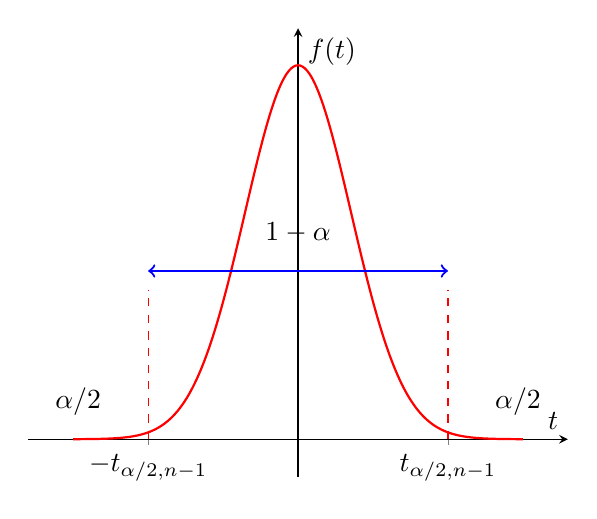
\begin{tikzpicture}
        \begin{axis}[
            axis lines=middle,
            enlargelimits=true,
            xlabel={$t$},
            ylabel={$f(t)$},
            xtick={-2, 2},
            xticklabels={$-t_{\alpha/2,n-1}$, $t_{\alpha/2,n-1}$},
            ytick=\empty,
            clip=false,
            domain=-3:3,
            samples=100,
            color=black
        ]
        \addplot [smooth, thick, red] {exp(-x^2)};
        \draw [dashed, red] (axis cs:-2,0) -- (axis cs:-2,0.4);
        \draw [dashed, red] (axis cs:2,0) -- (axis cs:2,0.4);
        \node at (axis cs:0,0.5) [above] {$1 - \alpha$};
        \node at (axis cs:-2.5,0.1) [left] {$\alpha/2$};
        \node at (axis cs:2.5,0.1) [right] {$\alpha/2$};
        \draw [<->, thick, blue] (axis cs:-2,0.45) -- (axis cs:2,0.45);
        \end{axis}
    \end{tikzpicture}
    \caption{Two sided inference with the student-t distribution.}
\end{figure}

We have seen that $\Bh\sim N(\B, \s^2(\X^\top\X)^{-1})$. Denote $(\X^\top\X)^{-1}=(e_{ij})_{i,j=1,\dots,p}$. We then have $\bh_j\sim N(\b_j, \s^2 e_{jj})$, so $\frac{\bh_j-\b_j}{\sqrt{e_{jj}}\s}\sim N(0,1)$. Since the variance is unknown, consider the statistic:
$$
    \frac{\bh_j-\b_j}{\sqrt{e_{jj}}\sh}
    =
    \frac{(\bh_j-\b_j)/\s\sqrt{e_{jj}}}{\sqrt{\frac{(n-p)\sh^2}{\s^2} / (n-p)}}.
$$
Recalling the properties of the estimators, we know that $\Bh, \sh^2$ are independent, that the numerator is $N(0,1)$-distributed and that $V=\frac{(n-p)\sh^2}{\s^2}\sim \chi^2_{n-p}$. Hence, we may conclude:
\begin{equation}
    \boxed{T = \frac{\bh_j-\b_j}{\sqrt{e_{jj}}\sh} \sim t_{n-p}}
\end{equation}
With this, we may constrict \term{confidence interval} by rewriting the inequalities in the expression:
$$
    \p{-t_{\frac{\alpha}{2},n-p} \leq \frac{\bh_j-\b_j}{\sqrt{e_{jj}}\sh} \leq t_{\frac{\alpha}{2}, n-p}} = 1-\alpha.
$$
We may also perform \term{hypothesis testing}. Consider the following test at significance level $\alpha$:
$$
    \mr{H}_0 : \b_j = 0, 
    \quad\quad\quad
    \mr{H}_1 : \b_j \ne 0.
$$
Under $H_0$ we have $T=\frac{\bh_j-\b_j}{\sqrt{e_{jj}}\sh} \sim t_{n-p}$. The \term{critical region} under two-sided alternative is:
$$
    \abs{T} \geq t_{\frac{\alpha}{2}, n-p} \Rightarrow \mr{H}_0 \textrm{ is rejected}.
$$

\TODO{R printout with explanation of culumns}

\TODO{Does R do one or two sided hypothesis test ???}

%%%%%%%%%%%%%%%%%%%%%%%%%%%%%%%%%%%%%%%%%%%%%%%%%%%%
%\subsection*{Lecture 12}
\subsection{Some notes on independence}

We sometimes use that plugging independente random variables through some functions result in new independent random variables. The theorem below tells us when this is okay. 

\begin{theorem}
    Suppose $X, Y$ are independent random variables and that $f, g$ are two measurable functions. Then $f(X), g(Y)$ are also independent. 
\end{theorem}

A \term{measurable function} is a function s.t. the preimages of Borel sets are measurable in the given probability space. In particular, continous functions are measurable.


%%%%%%%%%%%%%%%%%%%%%%%%%%%%%%%%%%%%%%%%%%%%%%%%%%%%
\subsection{Analysis of variance (ANOVA)}
The following theorem forms the basis on our discussion of ANOVA. 
\begin{theorem} \label{thm:ANOVA}
    Assuming the necesarry assumptions, we have the \term{ANOVA decomposition}:
    $$
    \boxed{
    \underset{\mr{SST}}{\underbrace{
        \sum_{i=1}^n (Y_i - \bar{Y})}} = 
    \underset{\mr{SSR}}{\underbrace{
        \sum_{i=1}^n (\hat{Y}_i - \bar{Y})}} + 
    \underset{\mr{SSE}}{\underbrace{
        \sum_{i=1}^n (Y_i - \hat{Y}_i)^2}}
    }
    $$
\end{theorem}
\begin{proof}
    We first split the sum as:
    \begin{align*}
        \sum_{i=1}^{n}\left(Y_{i}-\bar{Y}\right)^{2}
        &=\sum_{i=1}^{n}\left(Y_{i}-\hat{Y}_{i}+\hat{Y}_{i}-\bar{Y}\right)^{2}
        \\&= \sum_{i=1}^{n}\left(Y_{i}-\hat{Y}_{i}\right)^{2}+\sum_{i=1}^{n}\left(\hat{Y}_{i}-\bar{Y}\right)^2 
        +2{\sum_{i=1}^{n}\left(Y_{i}-\hat{Y}\right)\left(\hat{Y}_{i}-\bar{Y}\right)}.
    \end{align*}
    Using again the properties of the estimators, we find that the last sum is $0$:
    $$
        \sum_{i=1}^{n}\left(Y_{i}-\hat{Y}\right)\left(\hat{Y}_{i}-\bar{Y}\right)
        =
        \underbrace{\sum_{i=1}^{n} \overbrace{(Y_i-\hat{Y}_i)}^{\e_i}\hat{Y}_{i}}_{=\Eh^\top\hat{\Y}=0}
        -\bar{Y}\underbrace{\sum_{i=1}^{n}\left(Y_{i}-\hat{Y}\right)}_{=0 \textrm{ by property 2}}.
    $$
\end{proof}
The 3 sums are called \term{total sum of squares}, \term{regression sum of squares} and \term{error sum of squares} respectivelly. 
This decomposition motivates the following definition. 
\begin{definition}
    The part of the total variation due to the model is called the \term{coefficient of determination} or the \term{R2-score}:
    \begin{equation}
        \boxed{
            R^2 = \frac{\mr{SSR}}{\mr{SST}} \overset{\mr{thm}} = 1 - \frac{\mr{SSE}}{\mr{SST}}}        
    \end{equation}
\end{definition}
The R2-score is a measure of goodness-of-fit as it tells us how much of the variation in the data can be explained by the model. One may also prove another representation:
$$
    R^2 = \frac{\brac{\sum_{i=1}^n(Y_i-\bar{Y})(\hat{Y}_i-\bar{Y})}^2}{\sum_{i=1}^n(Y_i-\bar{Y})^2\sum_{i=1}^n(\hat{Y}_i-\bar{Y})}.
$$
This is the square of the empirical correlation between $\Y, \hat{\Y}$.

%%%%%%%%%%%%%%%%%%%%%%%%%%%%%%%%%%%%%%%%%%%%%%%%%%%%
%\subsection*{Lecture 13}
\subsubsection{Fictional model}
The following discussion will examine what happens when an explanatory variable is explained by the other explanatory variables. We introduce a \term{fictional model} using $x_{ij}$ as response for some fixed feature $j$. Wlog use feature $k$. The model is:
$$
    x_{i,k} = \alpha_0 + \alpha_1 x_{i,1} + \dots + \alpha_{k-1} x_{i, k-1} + \delta_i.
$$
As usual, we assume $\bs{\delta}=(\delta_1,\dots,\delta_n)^\top\sim N(0, \s^2\mI)$. We may then estimate $\bs{\alpha}=(\alpha_0,\dots,\alpha_{k-1})^\top$ and $\s^2$ by the usual $\hat{\bs{\alpha}}, \sh^2$ to obtain fitted $\hat{x}_{ik}$. We find the squared empirical correlation between $x_{i,k}$ and $\hat{x_{i,k}}$ as:
$$
    R_k^2 
    = \frac{\sum_{i=1}^n (\hat{x}_{ik}-\bar{x_k})^2}{\sum_{i=1}^n ({x}_{ik}-\bar{x_k})^2} 
    = \frac{\brac{\sum_{i=1}^n ({x}_{ik}-\bar{x_k})(\hat{x}_{ik}-\bar{x_k})}^2}
    {\sum_{i=1}^n ({x}_{ik}-\bar{x_k})^2\sum_{i=1}^n (\hat{x}_{ik}-\bar{x_k})^2}.
$$
We call it the coefficient of determination for $x_{ik}$ as response. Repeating the procedure for the remaining $x_{ij}, j=1,\dots,k-1$ we obtain $R_1^2,\dots,R_k^2$. It turns out that:
$$
    \var{\bh_j} = \frac{\s^2}{(1-R_j^2)\sum_{i=1}^n(x_{ij}-\bar{x}_j)}.
$$
So the more a variable is explained by the other, the higher the variance of the estimator.
%%%%%%%%%%%%%%%%%%%%%%%%%%%%%%%%%%%%%%%%%%%%%%%%%%%%
\subsubsection{Further expressions for the sums of squares}
Recall that $\mC, \mH$ are both symmetric an idempotent. For the total sum of squares, using that the centering matrix $\mC$ is idempotent, we obain:
\begin{align*}
    \mr{SST} = \sum_{i=1}^n(Y_i-\bar{Y})^2 = (\mC\Y)^\top(\mC\Y) = \Y^\top \mC \Y = \Y^\top\brac{\mI-\frac{1}{n}\one\one^\top}\Y.
\end{align*}
For the residual sum of squares we also need the fact that $\mH\x_i=\x_i$ for all columns of $\X$. This follows readily as $\mH\X=\X(\X^\top\X)^{-1}\X^\top\X=\X$. From this we have $\mH\one = \one$ as this is the first column of $\X$. 
\begin{align*}
    \mr{SSR} 
    &= \sum_{i=1}^n(\hat{Y}_i-\bar{Y})^2 
    = (\mC\mH\Y)^\top(\mC\mH\Y) 
    = \Y^\top\mH\mC\mH\Y 
    \\&= \Y^\top\brac{\mH-\frac{1}{n}\mH\one\one^\top\mH^\top}\Y 
    = \Y^\top\brac{\mH-\frac{1}{n}\one\one^\top}\Y.
\end{align*}
About the matrix $\mH-\frac{1}{n}\one\one^\top$, we note that it is symmetric, idempotent and of rank $p-1$:
$$
    \rank{\mH-\frac{1}{n}\one\one^\top} = \tr{\mH-\frac{1}{n}\one\one^\top} = \tr{\mH}-\frac{1}{n}\tr{\one\one^\top}=p-1.
$$
Finally, for the error sum of squares we obtain using that $\mI-\mH$ is symmetric and idempotent:
$$
    \mr{SSE} = \sum_{i=1}^n(\hat{Y}_i-Y_i)^2 = \Eh^\top\Eh = ((\mI-\mH)\Y)^\top(\mI-\mH)\Y = \dots = \Y^\top(\mI-\mH)\Y.
$$
%%%%%%%%%%%%%%%%%%%%%%%%%%%%%%%%%%%%%%%%%%%%%%%%%%%%
\subsection{F-test}
We first consider the hypothesis test:
$$
    \mr{H}_0 : \b_i = 0 \quad\forall i\in\{1,\dots,k\},
    \quad\quad\quad
    \mr{H}_1 : \b_i \ne 0 \textrm{ for at least one } i\in\{1,\dots,k\}.
$$
As usual we denote the significance level by $\alpha$. Our test statistic $F$ is:
\begin{align}
    \boxed{F = \frac{\mr{SSR}/(p-1)}{\mr{SSE}/(n-p)} \sim F_{p-1,n-p}}
\end{align}
And as usual the test is $F \geq f_{\alpha, p-1,n-p} \Rightarrow \mr{H}_0$ is rejected.
\begin{proof}
    \TODO{Uke 8}
\end{proof}

%%%%%%%%%%%%%%%%%%%%%%%%%%%%%%%%%%%%%%%%%%%%%%%%%%%%
\subsection{General F-test}
We set up a much more general problem. Let $A\in\R^{r\times p}$, $r<p$, $\mathrm{rank}(A)=r$, $\boldsymbol{d}\in\R^d$. We test the hypothesis:
$$
    \mr{H}_0 : A\B = \bs{d}, 
    \quad\quad\quad
    \mr{H}_1 : A\B \ne \bs{d}.
$$
Some special cases of this general setup are.
\begin{enumerate}[label=\textbullet]
    \item $r=1, d=0, A=(0, \dots, 1, \dots, 0)$ with $1$ at index $i$, gives the test 
    $$
        \mr{H}_0 : \b_i = 0, 
        \quad\quad\quad
        \mr{H}_1 : \b_i \ne 0.
    $$
    \item $r=1, d=0, A=(0, \dots, 1, \dots, -1, \dots, 0)$ with $1$ at index $i$ and $-1$ at index $j$, gives the test 
    $$
        \mr{H}_0 : \b_i = \b_j,
        \quad\quad\quad
        \mr{H}_1 : \b_i \ne \b_j.
    $$
    \item $r=k, d=\bs{0}\in\R^k, A=(\bs{0}, \mr{diag}(1))\in\R^{k\times p}$, gives the test 
    $$
        \mr{H}_0 : \b_i = 0 \quad\forall i\in\{1,\dots,k\},
        \quad\quad\quad
        \mr{H}_1 : \b_i \ne 0 \textrm{ for some } i\in\{1,\dots,k\}.
    $$
    This is the F-test of the previous section.
\end{enumerate}
%\subsection*{Lecture 14}
Let $\mathcal{B}$ be the space of $\B$ satisfying $\mr{H}_0$. The restricted problem is:
$$
    \Bh^R = \argmin_{\B\in\mathcal{B}}(\Y-\X\B)^\top(\Y-\X\B).
$$
Using lagrange multipliers and a bag of tricks, we obtain:
$$
    \Bh^R = \Bh - (\X^\top\X)^{-1}\bs{A}^\top(\bs{A}(\X^\top\X)^{-1}\mA^\top)^{-1}(\bs{A}\Bh-\bs{d}).
$$
Denoting $\Delta = \Bh-\Bh^R$, we find:
$$
    \mr{SSE}^R = \mr{SSE} + \Delta^\top\X^\top\X\Delta
$$
We claim that the under $\mr{H}_0$, we have
\begin{equation}
    \boxed{F = \frac{\brac{\mr{SSE}^R-\mr{SSE}} / r}{\mr{SSE}/(n-p)} \sim F_{r, n-p}}    
\end{equation}
\begin{proof}
    \TODO{Uke 8}
\end{proof}

%\subsection*{Lecture 15}
%... example ...

% \begin{figure}[H]\centering
%     \begin{tikzpicture}

%         % Axis
%         \begin{axis}[
%             no markers, 
%             domain=0:5, 
%             samples=100, 
%             axis lines*=left, 
%             xlabel=$F$, 
%             ylabel={}, 
%             height=6cm, 
%             width=10cm, 
%             xtick=\empty, 
%             ytick=\empty, 
%             enlargelimits=false, 
%             clip=false, 
%             axis on top,
%             grid = major,
%             color=black
%             ]
        
%             % F-distribution curve
%             \addplot+[smooth, thick] {x^2*exp(-x)};
            
%             % Critical value line and shaded region
%             \draw[thick] (axis cs:3,0) -- (axis cs:3,0.3);
%             \fill[pattern=north east lines, pattern color=black] (axis cs:3,0) -- (axis cs:5,0) -- (axis cs:5,0.05) -- (axis cs:3,0.05) -- cycle;
        
%             % Labels
%             \node at (axis cs:4,0.15) {$\alpha$};
%             \node[above] at (axis cs:3,0.3) {$f_{x,r_1,n-p}$};
%             \node[right] at (axis cs:4,0.4) {$H_0$ rejected};
%         \end{axis}
        
%         % Additional labels and annotations
%         \node[above right] at (8,3) {$F \geq f_{x,r_1,n-p}$};
        
%         \end{tikzpicture}
% \end{figure}


%%%%%%%%%%%%%%%%%%%%%%%%%%%%%%%%%%%%%%%%%%%%%%%%%%%%
\subsection{Transformations of data}
Some models common in applications are:
\begin{enumerate}
    \item $Y=\b_0+\b_1\frac{1}{x}+\varepsilon$
    \item $Y=\frac{1}{\b_0 x + \b_1 + \e}$
    \item $Y=\frac{x}{\b_0 x + \b_1 + x\e}$
\end{enumerate}
These can also be analysed using linear regression after undergoing some \term{transformations}, namelly:
\begin{enumerate}
    \item $\tilde{x}=\frac{1}{x} \leadsto Y=\b_0+\b_1\tilde{x}+\varepsilon$
    \item $\tilde{Y}=\frac{1}{Y} \leadsto \tilde{Y}=\b_0+\b_1{x}+\varepsilon$
    \item $\tilde{x}=\frac{1}{x},\tilde{Y}=\frac{1}{Y} \leadsto \tilde{Y}=\b_0+\b_1\tilde{x}+\varepsilon$
\end{enumerate}
We do not always know what form the model should have, which motivates the following section.

%%%%%%%%%%%%%%%%%%%%%%%%%%%%%%%%%%%%%%%%%%%%%%%%%%%%
\subsubsection{Box-Cox transformation}
The \term{Box-Cox transformation} is a power transform of the form:
\begin{equation}
    \boxed{
        u_{\lambda}(y) =
        \begin{cases}
            \begin{aligned}
                &\frac{y^\lambda-1}{\lambda}, && \text{if } \lambda \ne 0, \\
                &\ln{y}, && \text{if } \lambda = 0.
            \end{aligned}
        \end{cases}        
    }
\end{equation}
We immediatelly see that this requires $\Y>0$ the response $\Y$. To remedy negative $\Y$, simply shift them. To apply the transform, suppose that $\tilde{Y} = u_{\lambda}(Y)$ is normal and choose $\lambda$ which maximises the log-likelihood function. This turns out to not have analytic solution. 
To find the optimal $\lambda$, we therefore perform a \term{grid search}. In practice, we use the R function \texttt{boxcox}. 

%%%%%%%%%%%%%%%%%%%%%%%%%%%%%%%%%%%%%%%%%%%%%%%%%%%%
\subsubsection{Variance stabilising transformation}

Suppose $\mu_i=\ev{Y_i}$ and that $\var{Y_i}$ depends on $\mu_i$ by say $\var{Y_i}=h(\mu_i)$. Our goal is to transform by $\tilde{Y} = g(Y)$ so that the variance depends less on $\mu$. First order taylor expansion of $g(Y)$ around $\mu$ gives:
$$
    g(y) \approx g(\mu) + g'(\mu)(y-\mu).
$$ 
We find:
\begin{align*}
    \ev{g(Y)} &\approx g(\mu) + g'(\mu)\overbrace{(\ev{Y}-\mu )}^{=0} = g(\mu) 
    \\
    \var{g(Y)} &\approx \var{g(\mu) + g'(\mu)(Y-\mu)} = g'(\mu)^2\var{Y} 
\end{align*}
Choose $g(y)=\int_c^y \frac{1}{\sqrt{h(\mu)}}d\mu$. Then $g'(y) = \frac{1}{\sqrt{h(y)}}$ so $\var{g(Y)} = 1$.

\section{Model Analysis, Selection and Multiple Hypothesis Testing}
%\subsection*{Lecture 16}

%%%%%%%%%%%%%%%%%%%%%%%%%%%%%%%%%%%%%%%%%%%%%%%%%%%
\subsection{Model analysis}

Given a linear model, we can to some examination on the basis of visual analysis of residuals



\TODO{Example QQ plots ?}

\TODO{not homostochastic, not independent}
... transformed residuals free of trouble\dots
\TODO{long discussion of standardized / studentizes residuals ...}

%%%%%%%%%%%%%%%%%%%%%%%%%%%%%%%%%%%%%%%%%%%%%%%%%%%
\subsection{Model selection}
Some challenges when selecting model include:
\begin{enumerate}
    \item Unnecessary explanatory variables $\leadsto$ overfitting
    \item Missed relevant explanatory variables $\leadsto$ underfitting
    \item Quality of predictor $\centernot\iff$ Quality of estimator
\end{enumerate}

\TODO{example from 2017 exam}

Underfitting leads to biased estimation

Overfitting leads to greater variance in the estimators

%%%%%%%%%%%%%%%%%%%%%%%%%%%%%%%%%%%%%%%%%%%%%%%%%%%
%\subsection*{Lecture 17}
\subsubsection{Which model to choose}
Suppose $k$ covariates. Then we have $2^k$ possible models from maximal:
$$
    Y_i = \b_0+\b_1x_{i1} + \dots + \b_kx_{ik}.
$$
to minimal:
$$
    Y_i = \b_0.
$$
We want to arrive at a compromise between simplisity and goodness of fit. It is clear that the usual R2-score will not decrease by introducing additional variables, so we need to intruduce penalty for extra variables. Let $\sh^2$ be obtained from maximal model and $\mr{SSE}, p$ from the model of consideration.
\begin{enumerate}
    \item \term{Adjusted coefficient of determination}:
    $$
        \boxed{R^2_{\mr{adj}} = 1 - \frac{\mr{SSE} / (n-p-1)}{\mr{SST} / (n-1)} = 1 - (1-R^2)\frac{n-1}{n-p-1}}
    $$
    \item \term{Mallow's Cp parameter} (\hermetegn{Complexity parameter}):
    $$
        C_p = \frac{\mr{SSE}}{\sh^2} - n + 2p.
    $$
    \item \term{Akaibe information criterion}:
    $$
        \mr{AIC} = \frac{\mr{SSE}/n}{\sh^2} + 2\frac{p}{n}.
    $$
    \item \term{Bayesian information criterion}
    $$
        \mr{BIC} = \frac{\mr{SSE}/n}{\sh^2} + \ln{n}\frac{p}{n}.
    $$
\end{enumerate}
Note that for the 3 last options we want to minimise the statistic. In practice selection is done either with software or in to steps:
\begin{enumerate}
    \item For each $j=1,\dots,k$ choose the model with $j$ covariates of maximal R2-score. This gives $k$ models, so far not penalised.
    \item Consider these $k$ best models and choose `\hermetegn{best of the best} using one of the criteria. 
\end{enumerate}

%example...

%%%%%%%%%%%%%%%%%%%%%%%%%%%%%%%%%%%%%%%%%%%%%%%%%%%
%\subsection*{Lecture 18} % some 17
\subsection{Multiple hypothesis testing}
As before we consider the test:
$$
    \mr{H}_0 : \b_1=\dots=\b_k = 0.
$$
If this is now rejected, what about the individual tests $\b_j$? We can test individually using t-tests the hypothesis:
$$
    \mr{H}_0 : \b_j = 0.
$$
But if we have many parameters, $\p{\textrm{at least one type I error}}$ is large. In the worst case, for $m$ independent hypothesis we can compute this probability to be $1-(1-\alpha)^m$, which at significance $\alpha=0.05$ and $m=5, 20$ gives a probability $>0.22, >0.64$ respectivelly. We will now consider methods to resolve this issue. 
%The material is covered in more detail in \cite{Halle2017Multiple}.

%%%%%%%%%%%%%%%%%%%%%%%%%%%%%%%%%%%%%%%%%%%%%%%%%%%
\subsubsection{$p$-value is a random variable}

We recall that given an observation $t$ for the test statistiv $T$ we can compute the $p$-value, the probability of an equal of more extreme observation:
$$
    p(t) = \mathbb{P}_{\mathrm{H}_0} (T \geq t).
$$
Since $t$ is the observed value of a random variable, it is clear that the $p$-value is also random. The rejection criteria for $\mathrm{H}_0$ is: 
$$
    \mathrm{H}_0 \textrm{ is rejected} \Leftrightarrow p(t) \leq \alpha.
$$
An equivalent expression for the rejection criteria is:
$$
\mathrm{H}_0 \textrm{ is rejected} \Leftrightarrow t \geq t' \textrm{ with } \mathbb{P}_{\mathrm{H}_0} (T \geq t') = \alpha.    
$$
Hence we have
$$
    \mathbb{P}_{\mathrm{H}_0} (p(t) \leq \alpha) = \alpha,
$$
from which we conclude that under true $\mathrm{H}_0$, the $p$-value is uniformly distributed on $[0,1]$.

\begin{figure}[H]\centering
    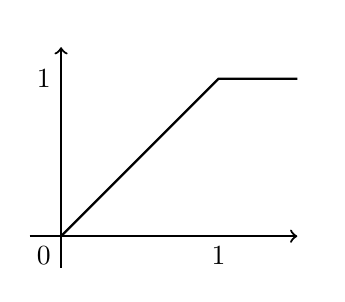
\begin{tikzpicture}[scale=2, thick]
        % Axes
        \draw[->, black] (-0.2, 0) -- (1.5, 0) node[right] {};
        \draw[->, black] (0, -0.2) -- (0, 1.2) node[above] {};
    
        % CDF
        \draw[thick] (0, 0) -- (1, 1) -- (1.5, 1);
    
        % Labels and ticks
        \draw (0, 0) node[below left] {0};
        \draw (1, 0) node[below] {1};
        \draw (1, 1) node[above right] {};
        \draw (0, 1) node[left] {1};
    
    \end{tikzpicture}
    \caption{Distribuon of the $p$-value.}
\end{figure}

%%%%%%%%%%%%%%%%%%%%%%%%%%%%%%%%%%%%%%%%%%%%%%%%%%%
\subsubsection{Testing $m$ hypothesis}
We begin by finding the $m$ $p$-values ($p_1,\dots,p_m$) corresponding to each hypothesis. We then need to choose the \term{local significance level} $\alpha_{\mr{loc}}$ and follow the rule that if $p$-value$\leq\alpha_{\mr{loc}}$ we reject the corresponding $\mr{H}_0$. We need to choose $\alpha_{\mr{loc}}$ such that the probability of at least one type I error is $\alpha$. The outcomes of our hypothesis test can be summarised by the table:
\begin{table}[htbp]
    \centering
    \caption{Multiple testing set-up}
    \begin{tabular}{cccc}
        \hline
         & H0 not rejected & H0 rejected & total \\
        \hline
        $\mr{H}_0$ true  & $U$   & $V$ & $m_0$\\
        $\mr{H}_0$ false & $T$   & $S$ & $m-m_0$\\
        total            & $m-R$ & $R$ & $m$\\
        \hline
    \end{tabular}
\end{table}
Note that we know $m$, the number of hypothesis, and the number $R$ of rejected hypothesis. Our goal is to control the \term{familywise error rate (FWER)}. This is the probability of at least one false positive finding:
$$
    \mr{FWER} = \p{V\geq 1} = 1- \p{V=0}.
$$
For independent hypothesis we find
\begin{align*}
    \mr{FWER} 
    &= 1- \p{p_1>\alpha_{\mr{loc}},\dots,p_m>\alpha_{\mr{loc}}}
    \\&= 1- \p{p_1>\alpha_{\mr{loc}}}\dots\p{p_m>\alpha_{\mr{loc}}}
    \\&= 1- (1-\alpha_{\mr{loc}})^m.
\end{align*}
If we for each hypothesis define the event:
$$
    R_j = \{\textrm{the j-th $\mr{H}_0$ is rejected but true}\} = \{p_j \leq \alpha_\mr{loc}\}.
$$
Then $\bar{R}_j=\{p_j > \alpha_{\mr{loc}}\}$ is the complementary event. We may write:
\begin{align*}
    \mr{FWER} 
    = \p{R_1\cup\dots\cup R_m} = 1 - \p{\bar{R}_1\cap\dots\cap \bar{R}_m}.
\end{align*}
We present two methods for choosing $\alpha_\mr{loc}$
\begin{enumerate}
    \item The \term{Bonferrony method} uses subadditivity to bound the $FWER$ by:
    $$
        \alpha = \mr{FWER} = \p{R_1\cup\dots\cup R_m} \leq \sum_{j=1}^m \p{R_j} = m \alpha_\mr{loc}.
    $$
    Hence the Bonferrony method is to let:
    \begin{equation}
        \boxed{\alpha_\mr{loc} = \frac{1}{m} \alpha}
    \end{equation}
    We make the following remarks:
    \begin{enumerate}
        \item This gives strong control (it works under any combination of true and false hypothesis).
        \item To get equality we need disjoint events / perfectly negativelly assosiated hypothesis.
        \item It is conservative: modelling dependencies may give lover requirement.
    \end{enumerate}
    \item For the \term{Šidák method} we make the assumption that we have \emph{independent tests}. Then we have seen that $\mr{FWER} = 1-(1-\alpha_{\mr{loc}})^m$. Hence the method is:
    \begin{equation}
        \boxed{\alpha_{\mr{loc}} = 1-(1-\alpha)^{1/m}}
    \end{equation}
    Again, we have strong control. The estimate is also exact when the tests are independent. It is conservative for positivelly dependent tests and liberal for negatively dependent tests. It is possible to show that the Šidák correction is always greater that the Bonferrony correction, so it is slighly less conservative; but we need to assume independence for exactness. 
\end{enumerate}

% ...
% example 2019 
% \dots
% example 2020

\section{ANOVA and Design of Experiment}
%%%%%%%%%%%%%%% Lecture 19 %%%%%%%%%%%%%%%
\subsection*{Lecture 19}

Example with three groups and their means ... rewrite to regression problem ...


 

\subsubsection*{Analysis of varance (ANOVA)}
p treatments, samples ...

 


%%%%%%%%%%%%%%% Lecture 20 %%%%%%%%%%%%%%%
\subsection*{Lecture  20}


... cont ... + brief on two way ANOVA

%%%%%%%%%%%%%%% Lecture 20 %%%%%%%%%%%%%%%
\subsection*{Lecture  21}
\subsection{Two level factorial design}

We suppose we have $k$ main factors $x_1,\dots,x_k$ making up a model of the form:
$$
    \Y=\beta_0 + \beta_1\x_1+\dots+\beta_k\x_k + \epsilon, \quad \epsilon\sim N(0, \sigma^2).
$$ 
Further we suppose a feature matrix $\X$ satisfying:
\begin{enumerate}
    \item Each column has entries $\pm 1$.
    \item The colomns are orthogonal, i.e. $\bf{1}^T\x_i=\sum_{i=1}^n x_{ij}=0$ and $\x_iT\x_j=n\delta_{ij}$. 
\end{enumerate}

This in particular implies that we have $\X^T \X = n I_n$. Using results from regression analysis, this significantly simplifies our estimators:

\TODO{expressions}

\begin{definition}
    The \term{main effect} of main factor $j$ is defined as:
    $$
        \textrm{effect}_j = \textrm{response at high level} - \textrm{response at low level} = 2\beta_j.
    $$
\end{definition}
The estimated effect is naturally
$$
    \widehat{\textrm{effect}_j} = \textrm{estimated response at high level} - \textrm{estimated response at low level} = 2\bh_j.
$$
To go from this to a $2^k$-design, we take into account interactions of the factors modelled as products of main factors:
$$
    Y = \b_0 + \b_1x_1+\dots+\b_kx_k + \b_{1,2}x_1x_2 + \dots+\b_{k-1,k}x_{k-1}k_{k}+\dots+\b_{1,2,\dots,k}x_1\cdots x_k.
$$
We extend the design matrix accordingly, and note that we still satisfy the assumptions. 

\TODO{example ?}

\subsubsection{Inference about effect}

Need inference about $\s^2$... cannot use estimator from multiple linear regression since for MLR we have $\sh^2=\frac{\textrm{SSE}}{n-p}$ and here $n=p$. We have to resort to one of two methods.

1. neglect some effects ... then these are normally dist ... use these as estimator \dots

2. Lenth's method ...



%%%%%%%%%%%%%%% Lecture 20 %%%%%%%%%%%%%%%
\subsection*{Lecture  22}



\subsubsection*{Resolution}

\term{resolution}


\subsubsection*{Blocking}


Vi tester en sitering \cite{test}.



% Bibiography and index of terms 
\newpage\printbibliography{}
\newpage\printindex{}
\end{document}